\section{A Dormant Subspace}
\label{sec:dormant}

\begin{figure*}[t]
\centering
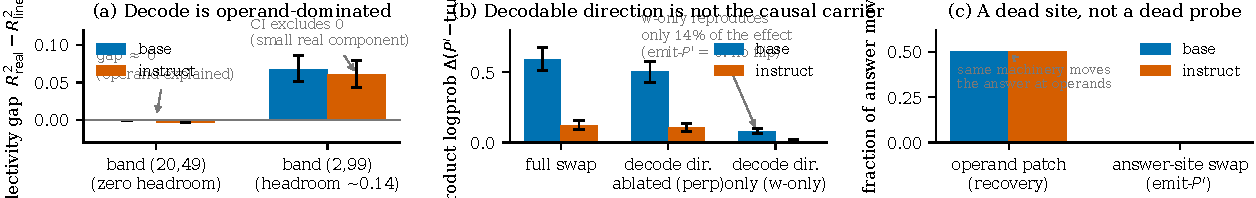
\includegraphics[width=0.82\textwidth]{figs/fig2_evidence.pdf}
\caption{The decodable answer-site subspace is dormant (bars/error bars are $95\%$ CIs).
\textbf{(a)} Selectivity gap (decode $R^2$ for \bc{} at ``$=$'' minus a linear-$(B,C)$ baseline):
at $[20,49]$ no headroom (gap $\approx 0$, operand-explained); at $[2,99]$ a small gap whose CI
excludes zero. \textbf{(b)} Causal share of a full-residual swap at the C4 ``$=$'' (base): ablating
the decode direction (perp) preserves most of the effect, the decode direction alone (w-only)
reproduces little, CIs non-overlapping; the swap flips no answers (emit-$P' = 0$). \textbf{(c)} The
dissociation as a fraction of the answer moved (two metrics): patching moves the answer at the
operand positions (recovery $0.50$) but the answer-site swap flips nothing, a dead \emph{site}, not
a dead probe. \textbf{(d)} Inject dose-response on the same axis: the C1 claim site is flat at
every dose (CIs bracket 0) while the C4 reference rises monotonically (base) yet never flips;
instruct's reference is weak and non-monotone.}
\label{fig:evidence}
\end{figure*}

The seductive story is that the product is computed and represented at the answer position but
not read out. We test it in three steps and reject it.

\paragraph{The product decodes (RQ2, correlational).}
A cross-validated probe recovers \bc{} from the ``$=$'' residual at $R^2 = 0.965$ (instruct),
$0.967$ (base) and the operand $B$ at $0.96$--$0.97$, with $B$ decodable at ``)'' at \emph{every} layer
including the last (instruct $0.98$, layer 31); taken alone this looks like a represented product.

\paragraph{But the decode is operand-dominated (RQ2, selectivity).}
Decodability of \bc{} need not mean the product is represented, since \bc{} is itself largely
linear in $B, C$ over a narrow band. We test this with a selectivity gap over a linear-$(B,C)$
baseline, but the gap test only has resolving power when the baseline leaves headroom:

\begin{proposition}[Headroom bound]
\label{prop:headroom}
For a target $g$, a decode probe with cross-validated $R^2_{\mathrm{real}}\le 1$, and a baseline
feature class $F$ with cross-validated $R^2_{F}$ on distribution $D$, the selectivity gap obeys
$\mathrm{gap}=R^2_{\mathrm{real}}-R^2_{F}\le 1-R^2_{F}$. The gap test therefore resolves at most the
\emph{headroom} $1-R^2_{F}$, so headroom is a design statistic that must be reported.
\end{proposition}

\noindent (Proof in Appendix~\ref{app:proof}; it applies to any derived quantity nearly linear in
its inputs on-distribution.) We compare \bc{} against the linear-$(B,C)$ baseline
(Figure~\ref{fig:evidence}a). At $[20,49]$ the baseline reaches $R^2 = 0.968$: by
Prop.~\ref{prop:headroom} the headroom is only $0.032$, so the test is a priori near-vacuous, and
indeed the gap is $-0.0002$. At $[2,99]$, where \bc{} is nonlinear in the operands (headroom
$0.135$), a small gap appears: $+0.068$, $95\%$ CI $[0.051, 0.086]$
(base) and $+0.060$, $[0.043, 0.079]$ (instruct), both excluding zero, and still positive at a
layer chosen by a C1-independent criterion (the C4 decode peak) rather than the C1 argmax. We flag that $[2,99]$ is
a harder regime where the parts fall below our $0.80$ floor (C4 $= 0.71$ base,
$0.73$ instruct), so we read it as a stress test, not a comfortably
in-scope measurement, and rest the headline on the band-independent causal null below. The
decode is operand-dominated ($\geq 0.94$ of it is reproduced by the linear-$(B,C)$ baseline,
$\approx 1.0$ at $[20,49]$) with at most a small operand-nonlinear component, consistent with a
weak product signal (behavior-tracking: C4 gap $>$ C1 gap, difference CI excludes zero).

\paragraph{And the decodable direction is causally inert (RQ3).}
We steer the ``$=$'' residual along the fitted direction to write a counterfactual product $P'$,
on held-out items. On the first-token metric the inject is null at every layer and matches
norm-matched random and shuffled controls (Appendix~\ref{app:steering}), but that metric is
non-discriminative between products. On the discriminative full-product metric, injecting at the
C1 ``$=$'' is flat at every dose $k \in \{1,2,4,8\}$ (CIs bracket zero) while the same inject at
the succeeding C4 ``$=$'' rises monotonically ($+0.08 \to +0.46$, every CI excluding zero, base)
yet never flips: the axis has dynamic range where the product is used and none at the failing
site, a dead direction rather than a dead instrument (emit-$P'$ stays zero throughout, a
saturating criterion, so we read the log-probability). A full-residual swap at the C4 ``$=$'',
\emph{where the model succeeds}, likewise fails to transplant the donor product (emit-$P' = 0$;
log-probability $+0.59$ at L19 where we decompose it, peak $+0.66$ at L23, still sub-flip); after
the swap the model still emits its \emph{own} correct answer at $0.90$--$0.95$ across L19--L31, so
the site is demonstrably bypassed. The product is thus not linearly resident at ``$=$'' even where
computed correctly, a fortiori at C1.
The one intervention that moves the answer is at the operand positions (recovery $0.50$; a
clean-answer recovery metric, a different readout and operation).

\paragraph{Certifying the illusion.}
We decompose the C4 swap effect into the decode direction and its orthogonal complement
(Figure~\ref{fig:evidence}b). Ablating the decode direction still leaves $+0.50$ (base), while
the decode direction alone contributes only $+0.08$, with non-overlapping CIs: $\approx 85\%$ of
the swap's (sub-flip) answer-effect survives removing the decodable direction (the swap moves only
$\approx 20\%$ of its magnitude along it). (The instruct swap effect is smaller, $+0.12$, its
decode-direction component not significantly positive; we report the decomposition for base.) We
use \emph{dormant} strongly: unlike a patch-potent-but-unused component, this direction moves
essentially nothing even when patched, present to a probe but invisible to computation
\citep{makelov-etal-2024-subspace}. Consistent with \citet{stolfo-etal-2023-mechanistic}
and \citet{nikankin-etal-2025-arithmetic}, the operands carry the signal but no sparse head set
reconstructs it (best head $< 0.02$); the value at ``$=$'' decodes and correlates yet cannot be
steered.

\paragraph{As a causal-abstraction claim.}
The full-residual swap is an interchange intervention \citep{geiger-etal-2021-causal} on the
``$=$'' residual: substituting a donor's representation should, if $B\!\cdot\!C$ is computed and
stored there, install the donor's answer. Interchange accuracy is $0$ (emit-$P'=0$) and the
original answer survives (emit-true $0.90$--$0.95$), so the hypothesis ``\bc{} is computed at
(``$=$'', layer $l$)'' fails as a causal-abstraction claim at every late $l$, even though the
correlational decode holds. Decodability and causal realization come apart at this node.

\paragraph{Hypotheses and evidence.}
Table~\ref{tab:hyp} collects the three readings of the failure against the committed evidence.

\begin{table}[t]
\centering
\footnotesize
\setlength{\tabcolsep}{3pt}
\begin{tabular}{@{}p{2.35cm}p{1.15cm}p{3.1cm}@{}}
\toprule
Hypothesis & Verdict & Evidence (committed) \\
\midrule
H1: product \emph{stored} at ``$=$'' & rejected & swap emit-$P'{=}0$, dose C1 flat, emit-true $0.90$--$0.95$ \\
H2: \emph{assembled} at readout from operands & supported & operand recovery $0.50$; $B$ decodable at every layer incl.\ 31; emit-true $0.90$--$0.95$ \\
H3: sparse answer-site circuit & no locus & best head $<0.02$; all heads inconclusive \\
\bottomrule
\end{tabular}
\caption{The composition failure adjudicated. Every cell traces to a committed file
(Appendix~\ref{app:battery}; \texttt{lateswap}, \texttt{dose\_response},
\texttt{operand\_localization}, \texttt{position\_decodability}, \texttt{head\_path\_patch}).}
\label{tab:hyp}
\end{table}

\paragraph{Predictions.}
H2 is falsifiable. It predicts that (i) ablating attention from ``$=$'' to the operand positions
during generation should destroy C4 accuracy, and (ii) few-shot recovery should act at the operand
positions rather than at ``$=$''. We state these as predictions, not results.
